\chapter{CMFD Acceleration}
\label{chap:cmfd}

In the previous section, the poor convergence of source iteration to solve the MOC equations was discussed. In this section, Course Mesh Finite Difference (CMFD) acceleration is introduced which allows for better convergence. During CMFD acceleration, a course mesh problem is solved that is consistent with the fine mesh MOC problem. Since the course mesh problem can be solved quickly, it can be fully converged and used to update the MOC solution allowing global behavior to be communicated in fewer iterations. This section shows how the CMFD equations are dervied from the fundamental multi-group transport equation and then the process of applying CMFD acceleration is discussed.

%%%%%%%%%%%%%%%%%%%%%%%%%%%%%%%%%%%%%%%%%%%%%%%%%%%%%%%%%%%%%%%%%%%%%%%%%%%%%%%
\section{General Description of CMFD}
\label{sec:cmfd-description}

- Discuss CMFD as a multi-grid approach (restriction / prolongation)

- Show mesh CMFD operates on

%%%%%%%%%%%%%%%%%%%%%%%%%%%%%%%%%%%%%%%%%%%%%%%%%%%%%%%%%%%%%%%%%%%%%%%%%%%%%%%
\section{Derivation of the CMFD Equations}
\label{sec:cmfd-derivation}

The CMFD equations can be derived from the fundamentals of multi-group transport. The general concept is to turn the transport equation, which is fundamentally based on angular fluxes into a diffusion problem which is fundamentally based on scalar fluxes averaged over some volume in the reactor. During this process, some approximations will be introduced. However, all of these approximations introduce no bias at convergence. Therefore they do not impact the solution accuracy. First recall the multigroup approximation given in Eq.~\ref{eqn:multi-group}:
\begin{equation}
	\mathbf{\Omega} \cdot \nabla \psi_{g}(\mathbf{r},\mathbf{\Omega}) + \Sigma_t^{g}(\mathbf{r}) \psi_{g}(\mathbf{r},\mathbf{\Omega}) = \frac{1}{4 \pi} \left( \frac{\chi_{g}\left(\mathbf{r}\right)}{k} \sum_{g'=1}^{G} \nu_{g'}\left(\mathbf{r}\right) \Sigma_f^{g'}\left(\mathbf{r}\right) \phi_{g'}\left(\mathbf{r}\right) + \, \sum_{g'=1}^G \,  \Sigma_{s}^{g' \rightarrow g}\left(\mathbf{r}\right) \phi_{g'}(\mathbf{r}) \right)
\end{equation}
To transform this equation into one based on the scalar fluxes $\phi_{g}(\mathbf{r})$ rather than the angular fluxes $\psi_{g}(\mathbf{r},\mathbf{\Omega})$, the equation is integrated over the enitre $4\pi$ angular space. In doing so, recall from Eq.~\ref{eqn:scalar-flux} that integral of angular flux over the entire angular space is simply the scalar flux. This leads to Eq.~\ref{eqn:angle_int_transport}.
\begin{equation}
	\int\displaylimits_{4 \pi} d\mathbf{\Omega} \,\mathbf{\Omega} \cdot \nabla \psi_{g}(\mathbf{r},\mathbf{\Omega}) + \Sigma_t^{g}\left(\mathbf{r}\right) \phi_{g}(\mathbf{r}) = \frac{\chi_{g}\left(\mathbf{r}\right)}{k} \sum_{g'=1}^{G} \nu_{g'}\left(\mathbf{r}\right) \Sigma_f^{g'}\left(\mathbf{r}\right) \phi_{g'}(\mathbf{r}) + \, \sum_{g'=1}^G \,  \Sigma_{s}^{g' \rightarrow g}\left(\mathbf{r}\right) \phi_{g'}(\mathbf{r})
	\label{eqn:angle_int_transport}
\end{equation}
Notice that only the streaming term has any dependence on the angular flux $\psi_{g}(\mathbf{r},\mathbf{\Omega})$. Since the angular variable $\mathbf{\Omega}$ is independent of the spatial variable $\mathbf{r}$, the gradient can be brought outside the integral in the streaming term as shown in Eq.~\ref{eqn:angle_int_transport_grad}.
\begin{equation}
	\nabla \cdot \int\displaylimits_{4 \pi} d\mathbf{\Omega} \,\mathbf{\Omega} \psi_{g}(\mathbf{r},\mathbf{\Omega}) + \Sigma_t^{g}\left(\mathbf{r}\right) \phi_{g}(\mathbf{r}) = \frac{\chi_{g}\left(\mathbf{r}\right)}{k} \sum_{g'=1}^{G} \nu_{g'}\left(\mathbf{r}\right) \Sigma_f^{g'}\left(\mathbf{r}\right) \phi_{g'}(\mathbf{r}) + \, \sum_{g'=1}^G \,  \Sigma_{s}^{g' \rightarrow g}\left(\mathbf{r}\right) \phi_{g'}(\mathbf{r})
	\label{eqn:angle_int_transport_grad}
\end{equation}
Next, the net current $J_g\left(\mathbf{r}\right)$ is defined as
\begin{equation}
J_g\left(\mathbf{r}\right) = \int\displaylimits_{4 \pi} d\mathbf{\Omega} \,\mathbf{\Omega} \psi_{g}(\mathbf{r},\mathbf{\Omega}).
\label{eqn:net_current}
\end{equation}
Insterting this definition and integrating the equation over an arbitrary volume $V$ leads to Eq.~\ref{eqn:vol_int_transport}.
\begin{equation}
	\int\displaylimits_{V} d\mathbf{r} \,\nabla \cdot J_g\left(\mathbf{r}\right) + \int\displaylimits_{V} d\mathbf{r} \, \Sigma_t^{g}\left(\mathbf{r}\right) \phi_{g}(\mathbf{r}) = \int\displaylimits_{V} d\mathbf{r} \, \left( \frac{\chi_{g}\left(\mathbf{r}\right)}{k} \sum_{g'=1}^{G} \nu_{g'}\left(\mathbf{r}\right) \Sigma_f^{g'}\left(\mathbf{r}\right) \phi_{g'}(\mathbf{r}) + \, \sum_{g'=1}^G \,  \Sigma_{s}^{g' \rightarrow g}\left(\mathbf{r}\right) \phi_{g'}(\mathbf{r}) \right)
	\label{eqn:vol_int_transport}
\end{equation}
Defining a volume $V_j$ for CMFD cell $j$ which is a composition of a finite and non-zero number of non-overlapping MOC source regions, the transport equation can be cast in terms of the fluxes and constant cross-sections for the MOC source regions $i$ with volumes $V_i$ as given in Eq.~\ref{eqn:cmfd_composition_moc}.
\begin{equation}
	\int\displaylimits_{V_j} d\mathbf{r} \,\nabla \cdot J_g\left(\mathbf{r}\right) + \sum_{i \in j} \int\displaylimits_{V_i} d\mathbf{r} \, \Sigma_t^{i,g} \phi_{g}(\mathbf{r}) = \sum_{i \in j} \int\displaylimits_{V_i} d\mathbf{r} \, \left( \frac{\chi_{i,g}}{k} \sum_{g'=1}^{G} \nu_{i, g'} \Sigma_f^{i,g'} \phi_{g'}(\mathbf{r}) + \sum_{g'=1}^G  \Sigma_{s}^{i, g' \rightarrow g} \phi_{g'}(\mathbf{r}) \right)
	\label{eqn:cmfd_composition_moc}
\end{equation}
Since the MOC equations are often solved for the average flux within source regions, $\overline{\phi_{i,g}}$, the transport equation can be re-written as:
\begin{equation}
	\int\displaylimits_{V_j} d\mathbf{r} \,\nabla \cdot J_g\left(\mathbf{r}\right) + \sum_{i \in j} \Sigma_t^{i,g} \overline{\phi_{i,g}} V_i = \sum_{i \in j} \left( \frac{\chi_{i,g}}{k} \sum_{g'=1}^{G} \nu_{i, g'} \Sigma_f^{i,g'} \overline{\phi_{i,g'}} V_i + \sum_{g'=1}^G   \Sigma_{s}^{i, g' \rightarrow g}\overline{\phi_{i,g'}} V_i \right)
\end{equation}
All of the variables given in this equation are present in the MOC equations except for the net current found in the streaming term. The bounding surface of CMFD cell $j$ is defined as $S_j$ with surface normal $\mathbf{n}$. Applying gauss-divergence theorem to the streaming term, it can be cast as a surface integral, shown in Eq.~\ref{eqn:cmfd_gauss_divergence}.
\begin{equation}
	\int\displaylimits_{S \in S_j} dS \, J_g\left(\mathbf{r}\right) \cdot \mathbf{n} + \sum_{i \in j} \Sigma_t^{i,g} \overline{\phi_{i,g}} V_i = \sum_{i \in j} \left( \frac{\chi_{i,g}}{k} \sum_{g'=1}^{G} \nu_{i, g'} \Sigma_f^{i,g'} \overline{\phi_{i,g'}} V_i + \sum_{g'=1}^G   \Sigma_{s}^{i, g' \rightarrow g}\overline{\phi_{i,g'}} V_i \right)
	\label{eqn:cmfd_gauss_divergence}
\end{equation}
In order to make the CMFD problem even less computationally intense, the group structure is coarsened. A group collapse is performed in which a given CMFD group $e$ is the incorportation of one or more MOC groups. To arrive at this relationship, the transport equation is summed over all MOC groups $g$ within the CMFD group $e$, shown in Eq.~\ref{eqn:cmfd_sum_groups}.
\begin{equation}
	\sum_{g \in e} \left( \int\displaylimits_{S \in S_j} dS \, J_g\left(\mathbf{r}\right) \cdot \mathbf{n} + \sum_{i \in j} \Sigma_t^{i,g} \overline{\phi_{i,g}} V_i \right) = \sum_{i \in j} \left( \frac{\sum_{g \in e} \chi_{i,g}}{k} \sum_{g'=1}^{G} \nu_{i, g'} \Sigma_f^{i,g'} \overline{\phi_{i,g'}} V_i + \sum_{g'=1}^G \left(\sum_{g \in e} \Sigma_{s}^{i, g' \rightarrow g} \right) \overline{\phi_{i,g'}} V_i \right)
	\label{eqn:cmfd_sum_groups}
\end{equation}
Similar to the process of forming multi-group cross-sections from continuous energy definitions in Chapter~\ref{chap:transport-theory}, CMFD cross-sections over coarse mesh and coarse group structures are defined in terms of the fine mesh MOC quantitites. The CMFD cross-sections are given the subscript $C$ and their defition are given in Equations $XX - YY$. 
\begin{equation}
	\chi_C^{j,e} = \frac{\sum_{i \in j} \left[ \left(\sum_{g \in e} \chi_{i,g} \right) \left(\sum_{g'=1}^{G} \nu_{i, g'} \Sigma_f^{i,g'} \overline{\phi_{i,g'}} V_i \right)\right]}{\sum_{i \in j} \sum_{g=1}^{G} \nu_{i, g} \Sigma_f^{i,g} \overline{\phi_{i,g}} V_i}
\end{equation}
\begin{equation}
	\nu_C^{j,e} \, \Sigma_{C,f}^{j,e} = \frac{\sum_{i \in j} \sum_{g \in e} \nu_{i, g} \Sigma_f^{i,g} \overline{\phi_{i,g}} V_i}{\sum_{i \in j} \sum_{g \in e} \overline{\phi_{i,g}} V_i}
\end{equation}
\begin{equation}
	\Sigma_{C,s}^{j, e' \rightarrow e} = \frac{\sum_{i \in j} \sum_{g'\in e'} \left(\sum_{g \in e} \Sigma_{s}^{i, g' \rightarrow g} \right) \overline{\phi_{i,g'}} V_i}{\sum_{i \in j} \sum_{g\in e} \overline{\phi_{i,g}} V_i}
\end{equation}
\begin{equation}
	\Sigma_{C,t}^{j, e} = \frac{\sum_{i \in j} \sum_{g \in e} \Sigma_{t}^{i, g} \overline{\phi_{i,g}} V_i}{\sum_{i \in j} \sum_{g\in e} \overline{\phi_{i,g}} V_i}
\end{equation}
Notice that these cross-sections involve a weighting over the MOC fluxes. Therefore the CMFD solution is limited in accuracy by the calculation of MOC scalar fluxes. At convergence, the MOC scalar fluxes are sufficiently accurate so that no significant approximation error is involved, allowing the CMFD solution to be entirely consistent. CMFD cell volumes $V_C^j$ and cell-averaged scalar fluxes $\phi_C^{j,e}$ are defined by Eq.~\ref{eqn:cmfd_volumes} and Eq.~\ref{eqn:cmfd_scalar_fluxes}, respectively.
\begin{equation}
	V_C^j = \sum_{i \in j} V_i
	\label{eqn:cmfd_volumes}
\end{equation}
\begin{equation}
\phi_C^{j,e} = \frac{\sum_{i \in j} \sum_{g \in e} \overline{\phi_{i,g}} V_i}{\sum_{i \in j} V_i}
\label{eqn:cmfd_scalar_fluxes}
\end{equation}
These definitions, along with the CMFD cross-section definitons, form the basis of the restriction component of CMFD acceleration. It is important to note that the CMFD mesh is significantly coarser - both in space and energy -- than the MOC mesh. A comparison of the spatial mesh is given in Figure~\ref{fig:cmfd-mesh} with the MOC mesh on the left. The depicted mesh are the actual mesh sizes used in the final results for this thesis. The MOC mesh is quite coarser than typical MOC mesh due to the use of a linear source approximation. The CMFD calculations use pin-cell sized mesh. Even with the coarse MOC mesh, the CMFD mesh is significantly coarser.
\begin{figure}[h!]
	\centering
	\begin{subfigure}{0.45\textwidth}
		\centering
		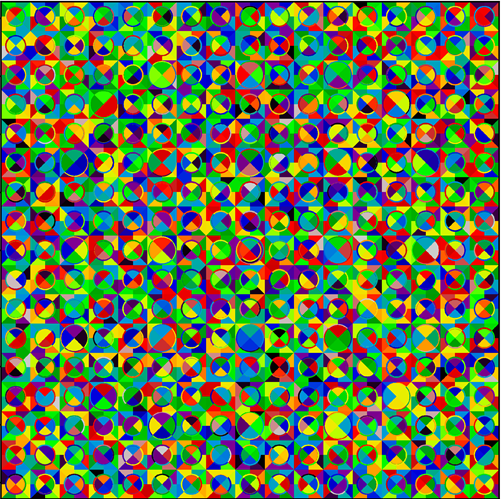
\includegraphics[width=\linewidth]{figures/moc_mesh.PNG}
		\caption{}
		\label{fig:cmfd-mesh-a}
	\end{subfigure}
	\begin{subfigure}{0.45\textwidth}
		\centering
		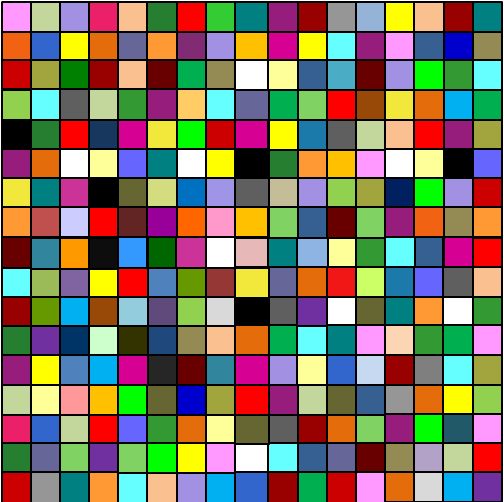
\includegraphics[width=\linewidth]{figures/cmfd_mesh.PNG}
		\caption{}
		\label{fig:cmfd-mesh-b}
	\end{subfigure}
	\caption[]{A depiction of the spatial mesh used in MOC (a) and CMFD (b) solvers. The mesh refinements correspond to those used in the final results for this thesis.}
	\label{fig:cmfd-mesh}
\end{figure}

For the energy condensation, the MOC calculations in this thesis use 70 energy groups whereas the CMFD solver uses 25 or less energy groups. The combination of coarse spatial mesh and coarse energy groups causes the CMFD problem size to be incredibly small in comparison with the MOC problem size. With the collapsed cross-sections on the coarse mesh, the CMFD transport equation looks very similar to the original mulit-group transport equation and is given in Eq.~\ref{eqn:cmfd_transport}.
\begin{equation}
	\frac{1}{V_C^j} \sum_{g \in e} \left( \int\displaylimits_{S \in S_j} dS \, J_g\left(\mathbf{r}\right) \cdot \mathbf{n} \right) + \Sigma_{C,t}^{j,e} \phi_C^{j,e} = \frac{\chi_C^{j,e}}{k} \sum_{e'=1}^{E} \nu_C^{j, e'} \Sigma_{C,f}^{j,e'} \phi_C^{j,e'} + \sum_{e'=1}^E  \Sigma_{C,s}^{i, e' \rightarrow e} \phi_C^{j,e'}
	\label{eqn:cmfd_transport}
\end{equation}
Returning to the streaming term, the entire surface $S_j$ of CMFD cell $j$ is partitioned into a finite number of partial surfaces $H$ that form an interface between cell $j$ and exactly one other CMFD cell. This allows the total net current of CMFD $j$ to be defined in terms of the sum over net currents over these interfacial surfaces as given in Eq.~\ref{eqn:cmfd_partial_surface_currents}.
\begin{equation}
	\frac{1}{V_C^j} \sum_{g \in e} \sum_{h=1}^H \left( \int\displaylimits_{S \in S_{j,h}} dS \, J_g\left(\mathbf{r}\right) \cdot \mathbf{n} \right) + \Sigma_{C,t}^{j,e} \phi_C^{j,e} = \frac{\chi_C^{j,e}}{k} \sum_{e'=1}^{E} \nu_C^{j, e'} \Sigma_{C,f}^{j,e'} \phi_C^{j,e'} + \sum_{e'=1}^E  \Sigma_{C,s}^{i, e' \rightarrow e} \phi_C^{j,e'}
	\label{eqn:cmfd_partial_surface_currents}
\end{equation}
The integrated net current over each interfacial surface for an MOC group $g$ can be cast in terms of angular fluxes using the definition given in Eq.~\ref{eqn:net_current} to produce the relationship in Eq.~\ref{eqn:interfacial_current_def}.
\begin{equation}
	\int\displaylimits_{S_{j,h}} dS \, J_g\left(\mathbf{r}\right) \cdot \mathbf{n} =  \int\displaylimits_{S \in S_{j,h}} dS \, \int\displaylimits_{4 \pi} d\mathbf{\Omega} \, \psi_{g}(\mathbf{r},\mathbf{\Omega}) \left(\mathbf{\Omega} \cdot \mathbf{n} \right)
	\label{eqn:interfacial_current_def}
\end{equation}
Figure~\ref{fig:cmfd-contact-surface} shows the geometric relationship between a given MOC track and CMFD surfaces. This shows that the surface area penetrated on surface $S_{j,h}$ by track $t$ can be calculated as $\delta A_{t} / \left(\mathbf{\Omega} \cdot \mathbf{n}\right)$.
\begin{figure}[h!]
	\centering
	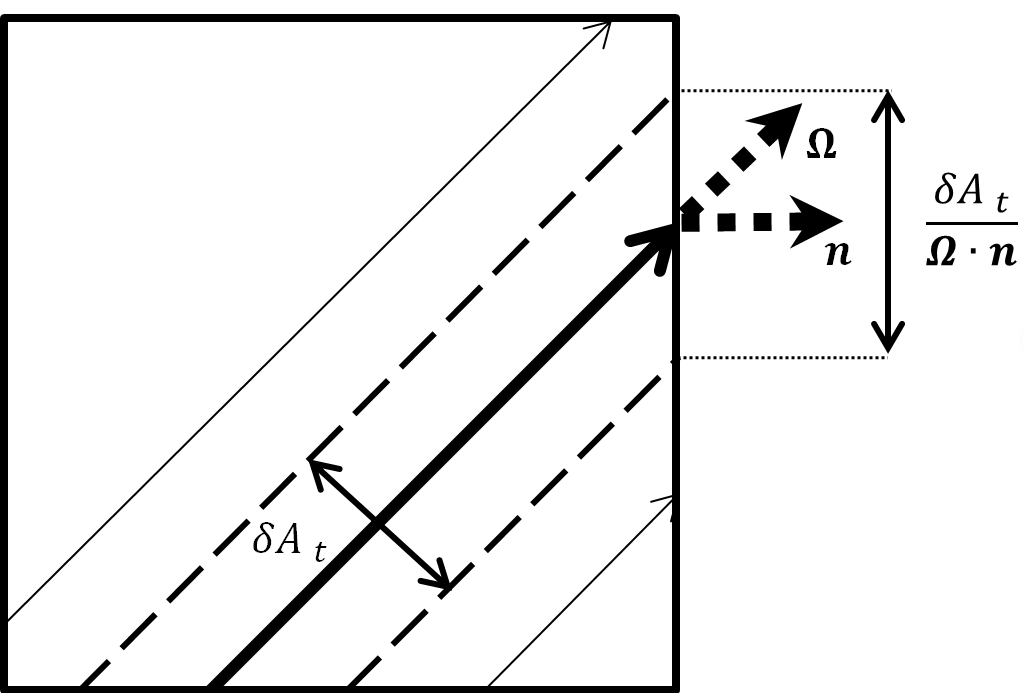
\includegraphics[width=0.5\linewidth]{figures/cmfd-contact-surface.PNG}
	\caption[]{A depiction of a CMFD surface with normal vector $\mathbf{n}$ being penetrated by a track with cross-sectional area $\delta A_{t}$ traveling in direction $\mathbf{\Omega}$. The area of the penetrated surface area is $\delta A_{t} / \left(\mathbf{\Omega} \cdot \mathbf{n}\right)$.}
	\label{fig:cmfd-contact-surface}
\end{figure}
With this geometric relationship in mind and factoring in angular weights from Eq.~\ref{eqn:weight-def}, the integrated net current over the interfacial surface can be calculated using Eq.~\ref{eqn:moc_net_current_calc}.
%\begin{equation}
%	\int\displaylimits_{S_{j,h}} dS \, J_g\left(\mathbf{r}\right) \cdot \mathbf{n} =  \sum_{(t,s) \in S_{j,h}} \frac{w_{t}}{\mathbf{\Omega} \cdot \mathbf{n}} \psi_{g}^{t,s}(s_{j,h}) \left(\mathbf{\Omega} \cdot \mathbf{n} \right)
%\end{equation}
\begin{equation}
	\int\displaylimits_{S \in S_{j,h}} dS \, J_g\left(\mathbf{r}\right) \cdot \mathbf{n} =  \sum_{(t,s) \in S_{j,h}} w_{i,t} \psi_{g}^{t,s}(s_{j,h})
	\label{eqn:moc_net_current_calc}
\end{equation}
Similar to the CMFD cross-sections, these currents are formed from the MOC calculation so are only approximate until convergence. Summing over all MOC groups $g$ within CMFD group $e$ gives a representation for the net current $\tilde{J}_{j,h,e}$ accross surface $h$ of cell $j$ for CMFD group $3$ in Eq.~\ref{eqn:cmfd_partial_current}.
\begin{equation}
	\tilde{J}_{j,h,e} = \sum_{g \in e} \sum_{(t,s) \in S_{j,h}} w_t \psi_{g}^{t,s}(s_{j,h})
	\label{eqn:cmfd_partial_current}
\end{equation}
It is important to note that these estimates rely on angular fluxes. Since the entire angular flux vector is not stored explicitly, as discussed in Section~\ref{sec:moc-solve}, when a CMFD surface is encountered during the MOC transport sweep, the contribution of angular fluxes along the track to the net current on the CMFD surface must be tallied. This is usually a relatively cheap operation, not adding much work to the transport sweep. With these calculated currents, the new transport equation is given in Eq.~\ref{eqn:transport_partial_current_1}.
\begin{equation}
	\frac{1}{V_C^j} \sum_{h=1}^H \tilde{J}_{j,h,e} + \Sigma_{C,t}^{j,e} \phi_C^{j,e} = \frac{\chi_C^{j,e}}{k} \sum_{e'=1}^{E} \nu_C^{j, e'} \Sigma_{C,f}^{j,e'} \phi_C^{j,e'} + \sum_{e'=1}^E  \Sigma_{C,s}^{i, e' \rightarrow e} \phi_C^{j,e'}
	\label{eqn:transport_partial_current_1}
\end{equation}
With this new representation of the transport equation, it is possible to solve for new scalar fluxes. However, this is not in the form of an eigenvalue problem since the streaming term has no dependence on the scalar flux. Physically, a relationship is indeed expected between the streaming term and scalar flux since high scalar flux indicates dense neutron population and hence more leakage out of the volume. This concept is very similar to diffusion theory. Therefore, new terms are introduced that relate the current to the scalar flux via diffusion coefficients. This is shown in Eq.~\ref{eqn:cmfd_current_repr}.
\begin{equation}
	\frac{\tilde{J}_{j,h,e}}{A_{j,h}} = - u(j,h) \hat{D}_{j,e} \left(\phi_C^{I(j,h),e} - \phi_C^{j,e}\right) - \tilde{D}_{j,h,e} \left(\phi_C^{I(j,h),e} + \phi_C^{j,e}\right)
	\label{eqn:cmfd_current_repr}
\end{equation}
The function $u(j,h)$ is the \textit{sense} of the surface $h$ on cell $j$, $A_{j,h}$ is the area of surface $S_{j,h}$, $\hat{D}_{j,e}$ is the surface diffusion coefficient, and $\tilde{D}_{j,h,e}$ is the nonlinear corrected diffusion coefficient. The inspiration first term involving $\hat{D}_{j,e}$ comes from diffusion theory. Specifically it can be calculated using Eq.~\ref{eqn:surf_diff_coef} under a CMFD uniform mesh assumption
\begin{equation}
	\hat{D}_{j,h,e} = \frac{2 D_{j,e} D_{I(j,h),e}}{\Delta \mathbf{r}_h \left( D_{j,e} + D_{I(j,h),e} \right)}
	\label{eqn:surf_diff_coef}
\end{equation}
where $\Delta \mathbf{r}_h$ is the distance between the CMFD cell and the interfacial surface $h$, the function $I(j,h)$ yields the neighboring CMFD cell of $j$ on surface $h$, and $D_{j,e}$ is the bulk diffusion coefficient of cell $j$ in group $e$. Due to the uniform mesh assumption, the distance between the centroid of cell $j$ and surface $h$ is the same as that of the neighboring cell $I(j,h)$. The bulk diffusion coefficients are deined in Eq.~\ref{eqn:cmfd_diff_coef}, with motivation from how diffusion coefficients are calculated in common nodal diffusion theory.
\begin{equation}
	D_{j,e} = \frac{\sum_{i \in j} \sum_{g \in e} \frac{1}{3\Sigma_{t}^{i, g}} \overline{\phi_{i,g}} V_i}{\sum_{i \in j} \sum_{g \in e} \overline{\phi_{i,g}} V_i}
	\label{eqn:cmfd_diff_coef}
\end{equation}
The sense $u(j,h)$ is calculated by Eq.~\ref{eqn:sense} where $\mathbb{1}$ is just the vector of ones in three dimensions and $\mathbf{n}_{j,h}$ is the normal vector of surface $S_{j,h}$. For a Cartesian uniform mesh, the sense is $+1$ if the surface is a positive $x$, $y$, or $z$ surface and $-1$ if it is a negative $x$, $y$, or $z$ surface.
\begin{equation}
u(j,h) = \frac{\mathbb{1} \cdot \mathbf{n}_{j,h}}{|\mathbb{1} \cdot \mathbf{n}_{j,h}|}
\label{eqn:sense}
\end{equation}
Lastly, the corrected diffusion coefficients $\tilde{D}_{j,h,e}$ are defined so that the relationship in Eq.~\ref{eqn:cmfd_current_repr} holds using currents and scalar fluxes calculated from the MOC iteration. This makes the CMFD calculation consistent with the MOC calculation and accurate at convergence. The calcualtion of the corrected diffusion coefficients therefore follows Eq.~\ref{eqn:cmfd_corr_dif_coef} where $\tilde{\phi}_C^{j,e}$ are the CMFD cell-averaged scalar fluxes calculated from the MOC iteration with the tilde indicating the quantity comes from the MOC calculation and does not change throughout the CMFD iterations.
\begin{equation}
	\tilde{D}_{j,h,e} = \frac{-u(j, h) \hat{D}_{j,h,e} \left(\tilde{\phi}_C^{I(j,h),e} - \tilde{\phi}_C^{j,e}\right) - \frac{\tilde{J}_{j,h,e}}{A_{j,h}}}{\tilde{\phi}_C^{I(j,h),e} + \tilde{\phi}_C^{j,e}}
	\label{eqn:cmfd_corr_dif_coef}
\end{equation}
Returning to balance equation and inserting the relationship for net current yields the new balance equation given in Eq.~\ref{eqn:cmfd_final_balance}.
\begin{equation}
\begin{split}
	\frac{1}{V_C^j} \sum_{h=1}^H A_{j,h} \left( - u(j, h) \hat{D}_{j,e} \left(\phi_C^{I(j,h),e} - \phi_C^{j,e}\right) - \tilde{D}_{j,h,e} \left(\phi_C^{I(j,h),e} + \phi_C^{j,e}\right) \right) + \Sigma_{C,t}^{j,e} \phi_C^{j,e} = \\
	\frac{\chi_C^{j,e}}{k} \sum_{e'=1}^{E} \nu_C^{j, e'} \Sigma_{C,f}^{j,e'} \phi_C^{j,e'} + \sum_{e'=1}^E  \Sigma_{C,s}^{i, e' \rightarrow e} \phi_C^{j,e'}
\end{split}
\end{equation}
Re-arranging terms in the balance equation and grouping by scalar flux yields the relationship in Eq.~\ref{eqn:cmfd_balance_grouped}.
\begin{equation}
	\begin{split}
		\left[\Sigma_{C,t}^{j,e} V_C^j + \sum_{h=1}^H A_{j,h} \left(u(j,h) \hat{D}_{j,e} - \tilde{D}_{j,h,e} \right) \right] \phi_C^{j,e} - \sum_{h=1}^H A_{j,h} \left( \tilde{D}_{j,h,e} + u(j,h) \hat{D}_{j,e} \right) \phi_C^{I(j,h),e} & \\ - \sum_{e'=1}^E  \Sigma_{C,s}^{i, e' \rightarrow e} V_C^j \phi_C^{j,e'} =
		\frac{\chi_C^{j,e}}{k} \sum_{e'=1}^{E} \nu_C^{j, e'} \Sigma_{C,f}^{j,e'} V_C^j \phi_C^{j,e'} & \\
	\end{split}
	\label{eqn:cmfd_balance_grouped}
\end{equation}
This can be written in terms of a matrix eigenvalue problem by defining a scalar flux vector $\Phi_C$ which incorporates all of the CMFD cell-averaged scalar fluxes $\phi_C^{j,e}$, a loss matrix $A$, and a multiplicative matrix $M$ in Eq.~\ref{eqn:cmfd_eigenvalue_problem}.
\begin{equation}
	A \Phi_C = \frac{1}{k} M \Phi_C
	\label{eqn:cmfd_eigenvalue_problem}
\end{equation}
This can be related to a regular eigenvalue problem by taking the inverse of $A$ as
\begin{equation}
	A^{-1} M \Phi_C = k \Phi_C.
\end{equation}
Any common eigenvalue solver can be used to solve this system. In this thesis, simple power iteration is employed. More details on practical implementation aspects of CMFD in this thesis are given in Chapter~\ref{chap:cmfd-optimize}.

Once the CMFD equations are solved, the solution is used to update MOC fluxes, hence producing a new source on the next iteration. The updating of MOC fluxes is the prolongation step of the CMFD process. There are a variety of ways for which the CMFD fluxes can be updated. One simple approach is just updating all MOC fluxes in source region $i$ and MOC group $g$ encompassed by CMFD cell $j$ and CMFD group $e$ by appliying Eq.~\ref{eqn:cmfd_simple_prolongation}:
\begin{equation}
\phi_{i,g}^{\text{new}} = \phi_{i,g}^{\text{old}} \, \frac{\phi_{C, \, \text{new}}^{j,e}}{\phi_{C, \, \text{old}}^{j,e}}
\label{eqn:cmfd_simple_prolongation}
\end{equation}
where $\phi_{i,g}^{\text{new}}$ refers to the updated MOC flux after prolongation, $\phi_{i,g}^{\text{old}}$ refers to the MOC flux before prolongation, $\phi_{C, \, \text{old}}^{j,e'}$ refers to the CMFD cell-averaged flux at the start of the CMFD solution (calculated directly from the MOC fluxes), and $\phi_{C, \, \text{new}}^{j,e'}$ refers to the CMFD cell-averaged flux at convergence of the CMFD solution.

\section{Application of CMFD for MOC Convergence Acceleration}
Now that the theoretical background has been discussed in forming the CMFD equation, the use of CMFD related to the MOC problem is discussed.


Insert flow diagram:
Guess initial scalar flux distribution and boundary angular fluxes
->
Compute sources
Solve MOC equations for the source distribution
Collapse cross sections, currents, form CMFD equations
Solve CMFD equations
Update scalar fluxes, k
<-